\documentclass[20pt]{article}

\usepackage[english]{babel}
\usepackage[utf8x]{inputenc}
% \usepackage{amsmath}
\usepackage{graphicx}
\usepackage[margin=0.8in]{geometry}

\title{AS205:Ocean Dynamics(Assignment 4)}
\author{Parag Shende}

\begin{document}
\maketitle
\hrule

\section*{Introduction}

We describe the seasonal means of the wind stress($\tau_{x}$ and $\tau_{y}$) and its curl in the Bay of Bengal and Arabian Sea. This is 
undertaken to study the spatial and temporal patterns of the two fields. The seasonal means are constructed for the year 2022.

\section*{Datasets}

The datasets used in this analysis is as follows:

\begin{itemize}
    \item \textbf{Sea Surface Eastward velocity(SSU)} : ASCAT data.
    \item \textbf{Sea Surface Northward velocity(SSV)} : ASCAT data.
\end{itemize}

\section*{Methodology}

The datasets are choosen for the domain of $40^{\circ} E$ to $100^{\circ}E$ and $0^{\circ} N$ to $25^{\circ} N$. This covers the
North Indian ocean. We then calculate the seasonal mean with the following seasons:
\begin{itemize}
    \item \textbf{Summer Monsoon} : June, July, August, September(JJAS)
    \item \textbf{Winter Monsoon} : November, December, January, February(NDJF)
\end{itemize}

The wind stress is calculated as follows:
\begin{center}
    $\tau_{x} = \rho*C_{d}*Umag*U$

    $\tau_{y} = \rho*C_{d}*Umag*V$    
\end{center}

where,
$\tau_{x}$ and $\tau_{y}$ are the wind stress in zonal and meridional direction respectively. 

$\rho_a$ is the density of the air (taken to be $1.12 \frac{kg}{m^{3}}$). 

$C_d$ is the drag coefficien taken to be
\begin{center}
    $C_{d} = 0.001*(0.46 + 0.14*Umag)$ ($Umag > 15.$)

    $C_{d} = 2.63*10^{-3}$ ($Umag < 15.$)
\end{center}


$Umag$ is the magnitude of the velocity vector

$U, V$ are the surface zonal and meridional velocities respectively.

The curl of wind stress is given by:
\begin{center}
    $\nabla\times\tau = \frac{\partial \tau_{y}}{\partial x} - \frac{\partial \tau_{x}}{\partial y}$
\end{center}

We contrast the differences in spatial and temporal features in the wind stress and curl of wind stress fields for the 
Arabian Sea and Bay of Bengal. 

\section*{Sea Surface Stress}

\subsection*{Summer Monsoon}

\begin{figure}
    \centering
    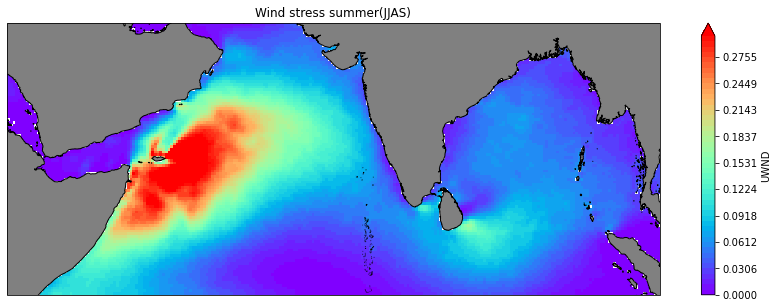
\includegraphics[width=0.88\textwidth]{wind_stress_summer.png}
    \caption{Wind stress in summer in $N/m^{2}$}
\end{figure}

\begin{itemize}
    \item The seasonal mean for summer is plotted in Figure 1. 
    \item The Maximum wind stress is observed near the Somali current region and east of Sri Lanka.
    \item The Arabian sea is dominanted by high wind stress which is indicative of the winds prevalent in the summer monsoon period.
    \item The Bay of Bengal is relatively calmer and high stress regions occur south-west of it.
\end{itemize}

\subsection*{Winter Monsoon}

\begin{figure}
    \centering
    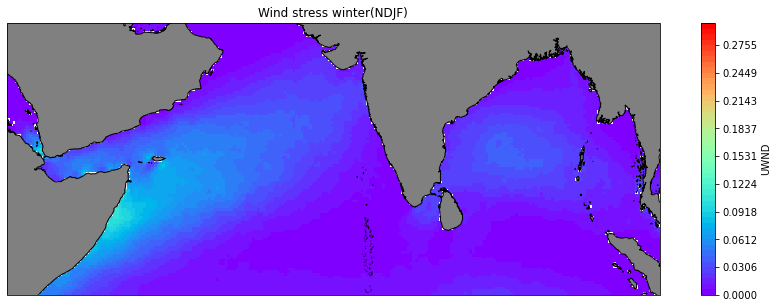
\includegraphics[width=0.88\textwidth]{wind_stress_winter.png}
    \caption{Wind stress in winter in $N/m^{2}$}
\end{figure}

\begin{itemize}
    \item The seasonal mean for winter is plotted in Figure 1. 
    \item The Maximum wind stress is again observed near the Somali current region.
    \item The south-west monsoon winds have died down and hence the whole of Arabian Sea is calmer as compared to its climatology in summer.
    \item The North Indian ocean on a whole is calmer in winter monsoon than in summer.
\end{itemize}

\section*{Curl of wind stress}

\subsection*{Summer Monsoon}

\begin{figure}
    \centering
    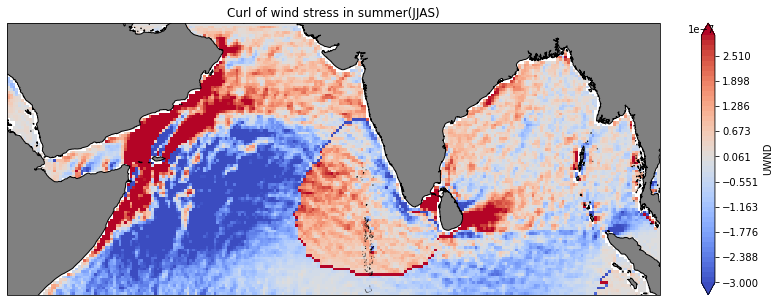
\includegraphics[width=0.88\textwidth]{curl_summer.png}
    \caption{Curl of wind stress in summer in $N/m$}
\end{figure}

\begin{itemize}
    \item We see that the curl of wind stress is positive near the Somali jet during summer.
    \item East and South-east of Sri Lanka is another large region of positive curl of wind stress. 
    \item The Bay of Bengal has lower value of curl than Arabian Sea.
\end{itemize}

\subsection*{Winter Monsoon}

\begin{figure}
    \centering
    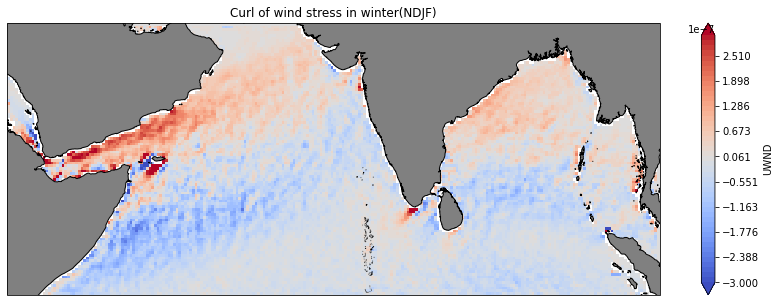
\includegraphics[width=0.88\textwidth]{curl_winter.png}
    \caption{Curl of wind stress in winter in $N/m$}
\end{figure}

\begin{itemize}
    \item The curl is weaker than compared to summer in all the regions.
    \item The curl is higher in Arabian sea as compared to Bay of Bengal.
\end{itemize}

\section*{Conclusions}

\begin{itemize}
    \item We compared the seasonal means of SST and SSS for northern Indian ocean.
    \item On an average the Arabian sea is saltier than the Bay of Bengal. This is primarly due to large freshwater influx in the bay.
    \item The Arabian sea is cooler than the Bay of Bengal as strong stratification in the bay prevents the deepening of mixed layer and hence the shortwave heat is surface trapped.
\end{itemize}

\end{document}